\documentclass{article}
\linespread{1.7}
\usepackage[letterpaper, margin=0.7in]{geometry}
\usepackage{graphicx}
\usepackage{amsmath}
\usepackage{subfig}
\usepackage[dvipsnames]{xcolor}

\title{Midterm 1}
\author{Yue Huang}

\begin{document}
\maketitle

\section{K-means}
\subsection{Euclidean distance}
\begin{enumerate}
\item
for each of data points, calculate euclidean distance to the centers $A (-3,-1)$ and $B(2,1)$, $D(x_i, c_j) = \|x_i - c_j\|^2$. After one iteration, the distance matrix and their assignments are below:

\medskip
\begin{tabular}{l|c|r|b}
x_i & D(x_i,A) & D(x_i,B) & assignment\\
\hline
1 (2,2)& 34 & 1 & B\\
2 (-1,1)& 8 & 9 &A\\
3 (3,1)&40&1 & B\\
4 (0,-1) &9&8 & B\\
5 (-2,-2) &2&25 & A
\end{tabular}

\item
then update the centers by averaging all the points within that center: 

new A = $\frac{1}{2} [(-1,1) + (-2,-2)] = (-1.5, -0.5)$

new B = $\frac{1}{3} [(2,2) + (3,1) + (0,-1)] = (-1.67, 0.67)$

\medskip
\item
let's go on to the 2nd iteration, the distance matrix and their assignment are below:

\medskip
\begin{tabular}{l|c|r|b}
x_i & D(x_i,A) & D(x_i,B) & assignment\\
\hline
1 (2,2)& 18.5 & 1.89 & B\\
2 (-1,1)& 2.5 & 7.22 & A\\
3 (3,1)& 22.5 & 1.89 & B\\
4 (0,-1) & 2.5 & 5.56 & A\\
5 (-2,-2) & 2.5 & 20.56 & A
\end{tabular}

\medskip
new A is (-1, -0.67), new B is (2.5, 1.5).
k-means algorithm will converge and terminate when the centers and assignments do not change. But we can clearly see that the assignments have been changed in the 2nd iteration, so it will not terminate in one step. Actually it will terminate in 3 steps.
\end{enumerate}

\subsection{Mahanttan distance}
\begin{enumerate}
\item
for each of data points, calculate Manhattan distance to the centers $A (-3,-1)$ and $B(2,1)$, $D(x_i, c_j) = \sum |x_i - c_j| $. After one iteration, the distance matrix and their assignments are below:

\medskip
\begin{tabular}{l|c|r|b}
x_i & D(x_i,A) & D(x_i,B) & assignment\\
\hline
1 (2,2)& 8 & 1 & B\\
2 (-1,1)& 4 & 3 &B\\
3 (3,1)& 8 & 1 & B\\
4 (0,-1) &3&4 & A\\
5 (-2,-2) &2&7 & A
\end{tabular}

\item
then update the centers by averaging all the points within that center: 

new A = $\frac{1}{2} [(0,-1) + (-2,-2)] = (-1, -1.5)$

new B = $\frac{1}{3} [(2,2) + (-1,1) + (3,1)] = (1.33, 1.33)$

\medskip
\item
let's go on to the 2nd iteration, the distance matrix and their assignment are below:

\medskip
\begin{tabular}{l|c|r|b}
x_i & D(x_i,A) & D(x_i,B) & assignment\\
\hline
1 (2,2)& 6.5 & 1.33 & B\\
2 (-1,1)& 2.5 & 2.67 & A\\
3 (3,1)& 6.5 & 2 & B\\
4 (0,-1) & 1.5 & 3.67 & A\\
5 (-2,-2) & 1.5 & 6.67 & A
\end{tabular}

\medskip
new A is (-1, -0.67), new B is (2.5, 1.5). k-means algorithm will converge and terminate when the centers and assignments do not change. But we can clearly see that the assignments have been changed in the 2nd iteration, so it will not terminate in one step. Actually it converges in 3 steps.
\end{enumerate}

\section{Spectral clustering}
I constructed undirected neighborhood graphs (breaking ties randomly) by connecting each point's 2 nearest neighbors. so a pair (i, i') is in adjacency matrix if point i is within 2 nearest neighbors of i', or vice-versa. Then we give the edge weight $w_{ii'} = exp(-\|x_i - x_j\|)$ . Here I assume we are evaluating the edge weight by euclidean distance. So specifically, $w_{ii'} = exp(-d_{ij})$, where $d_ij = \sqrt {\sum _{i=1}^{n}(q_{i}-p_{i})^{2}}$. 

Supposed the point numbers are marked respectively:

\begin{center}
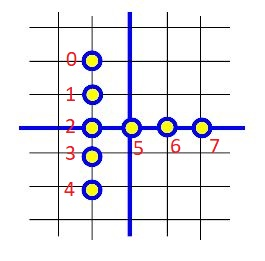
\includegraphics{figure2.JPG}
\end{center}

So the resulting neighborhood graphs for each point respectively are:

\textcolor{red}{0} - 1 - 2; \quad 0 - \textcolor{red}{1} - 2; \quad 1 - \textcolor{red}{2} - 5; \quad 2 - \textcolor{red}{3} - 4;

2 - 3 - \textcolor{red}{4}; \quad 2 - \textcolor{red}{5} - 6; \quad 5 - \textcolor{red}{6} - 7; \quad 5 - 6 - \textcolor{red}{7};

Therefore the adjacency matrix A is
\renewcommand{\arraystretch}{0.7}
$$
A = 
\begin{bmatrix}
0&1&1&0&0&0&0&0\\
1&0&1&0&0&0&0&0\\
1&1&0&1&1&1&0&0\\
0&0&1&0&1&0&0&0\\
0&0&1&1&0&0&0&0\\
0&0&1&0&0&0&1&1\\
0&0&0&0&0&1&0&1\\
0&0&0&0&0&1&1&0\\
\end{bmatrix}
$$

Our weighted adjacency matrix is therefore:
$$
W = 
\begin{bmatrix}
0&e^{-1}&e^{-2}&0&0&0&0&0\\
e^{-1}&0&e^{-1}&0&0&0&0&0\\
e^{-2}&e^{-1}&0&e^{-1}&e^{-2}&e^{-1}&0&0\\
0&0&e^{-1}&0&e^{-1}&0&0&0\\
0&0&e^{-2}&e^{-1}&0&0&0&0\\
0&0&e^{-1}&0&0&0&e^{-1}&e^{-2}\\
0&0&0&0&0&e^{-1}&0&e^{-1}\\
0&0&0&0&0&e^{-2}&e^{-1}&0\\
\end{bmatrix}
$$

And D is a diagonal matrix of W, where $d_{ii'} = \sum_{j=1}^m w_{ij}$. The graph Laplacian is L = D - W. 
$$
L = 
\begin{bmatrix}
e^{-1}+e^{-2}&-e^{-1}&-e^{-2}&0&0&0&0&0\\
-e^{-1}&2e^{-1}&-e^{-1}&0&0&0&0&0\\
-e^{-2}&-e^{-1}&3e^{-1}+2e^{-2}&-e^{-1}&-e^{-2}&-e^{-1}&0&0\\
0&0&-e^{-1}&2e^{-1}&-e^{-1}&0&0&0\\
0&0&-e^{-2}&-e^{-1}&e^{-1}+e^{-2}&0&0&0\\
0&0&-e^{-1}&0&0&2e^{-1}+e^{-2}&-e^{-1}&-e^{-2}\\
0&0&0&0&0&-e^{-1}&2e^{-1}&-e^{-1}\\
0&0&0&0&0&-e^{-2}&-e^{-1}&e^{-1}+e^{-2}\\
\end{bmatrix}
$$

Then we can perform eigen-decomposition of L. Find 2 eigenvectors corresponding to 2 smallest eigenvalues. 
After some calculation, the 2 smallest eigenvalue are $6.99\times10^{-18}$ and $1.16\times10^{-1}$, with corresponding eigenvectors $v_1, v_2$. Then we will perform k-means algorithm on
$$
Z = (v_1, v_2) =  
\begin{bmatrix}
0.35&-0.31\\
0.35&-0.27\\
0.35&-0.14\\
0.35&-0.27\\
0.35&-0.31\\
0.35&0.26\\
0.35&0.49\\
0.35&0.56
\end{bmatrix}
$$

by treating each row as new data point, and cluster the original data by labels assigned to Z's data point.

The resulting two clusters are labeled with blue and red colors:
\begin{center}
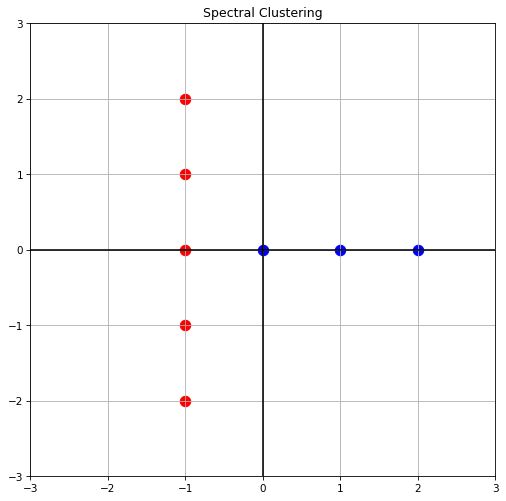
\includegraphics[scale=0.5]{result.png}
\end{center}

\section{Principal Component Analysis}
\subsection{}
To find the first principal direction, we need to find the eigenvector corresponding to the largest eigenvalue for the covariance matrix of data.

Our data X is
$$
X =  
\begin{bmatrix}
4&-2&4\\
5&-3&5\\
2&0&2\\
3&-1&3
\end{bmatrix}
$$

Our mean $u$ for data X is $u = \frac{1}{m} \sum_{i=1}^m x_i = [ 3.13, -1.34, 3.13]$. And the standard deviation for data is $\sigma = [ 1.12, 1.12, 1.12]$

Then the normalized covariance matrix C from normalized data is $C' = \frac{1}{m} \sum_{i=1}^m (x_i / \sigma - u')(x_i / \sigma - u')^T$.
$$
C' =  
\begin{bmatrix}
1&-1&1\\
-1&1&-1\\
1&-1&1
\end{bmatrix}
$$

Next, compute the eigenvector $w_1$ of $C'$ corresponding to the largest eigenvalue $\lambda_1$. Then $w_1$ is the first principal direction.
$$
w_1 = [0.577, -0.577, 0.577]^T
$$

\subsection{}

The reconstruction error in terms of variance can be directly computed from the eigenvalues of covariance matrix.

Because for given data points $x = (x_1, ..., x_m) \quad x\in R^n$, we need to find $w = (w_1, ... ,w_d) \in R^n, d < m$ such that the variance (or variation) of the data along direction w is maximized. The reconstruction error is then variances on the rest of the directions, namely, $(w_d, ... ,w_m)$ because we lose them due to missing components. The objective function is: 
$$
MAX_{w} \quad \frac{1}{m} \sum_{i=1}^d \sum_{i=1}^m (w_i^T x_i - w_i^T u)^2
=\sum_{i=1}^d w_i^T \{ \sum_{i=1}^m \frac{1}{m}(x_i - u)(x_i - u)^T \} w_i = \sum_{i=1}^d w_i^T C w_i
$$

\medskip
For covariance matrix C, we have $Cw = \lambda w $, so $\lambda = w^T Cw$.

\medskip
The maximization problem becomes maximizing the sum of largest eigenvalues of matrix C - max $\sum_{i=1}^d \lambda_i$.

This is equivalent to minimizing $\sum_{i=d+1}^m \lambda_i$. 

So our reconstruction error = $\sum_{i=d+1}^m \lambda_i$.

\medskip
From (a), we calculate eigenvalues $\lambda = [3.00, 2.21\times10^{-16}, 0.00]$, and $\lambda_1 = 3.00$.

So the first principal component explains all of the variances of the original data X.

\textbf{So our reconstruction error is $2.21\times10^{-16} \approx 0$, about 0 in this case.}

\subsection{}

\begin{centering}
\begin{figure}[h]%
    \centering
    \subfloat{{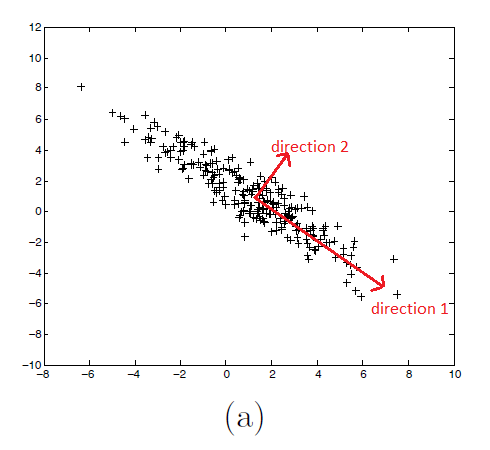
\includegraphics[width=6cm]{Q3(a).PNG}}}%
    \qquad
    \subfloat{{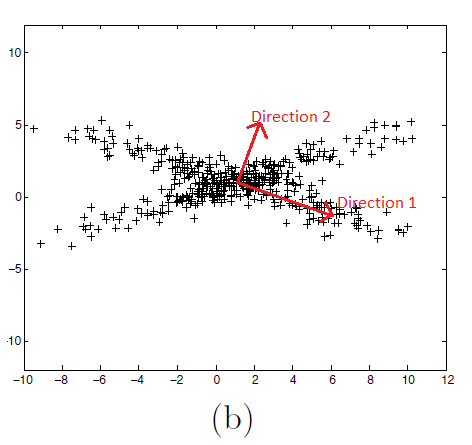
\includegraphics[width=6cm]{Q3(b).PNG}}}%
\end{figure}
\end{centering}

\section{PCA for face recognition}
\subsection{eigenfaces}

\begin{figure}[h!]
\centering
  \caption{Subject 01}
  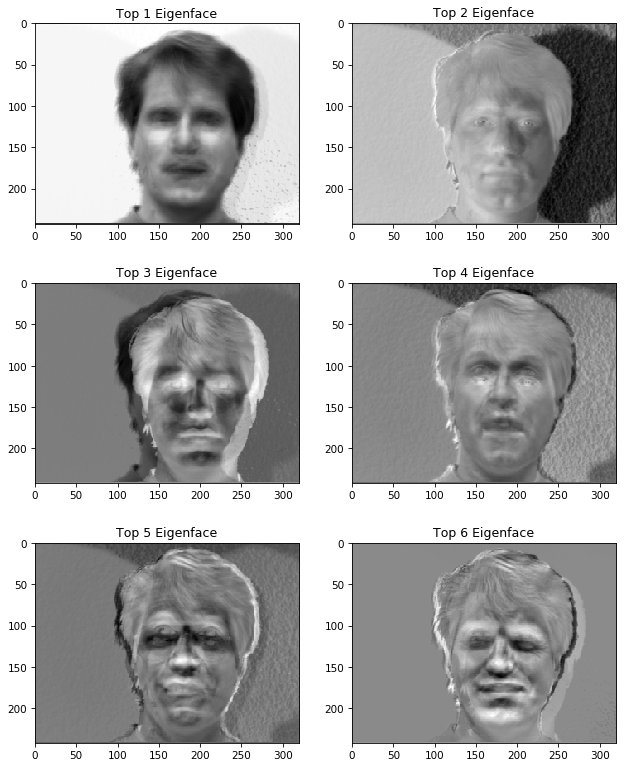
\includegraphics[scale = 0.36]{subject01.png}
\end{figure}

\begin{figure}[h!]
\centering
  \caption{Subject 14}
  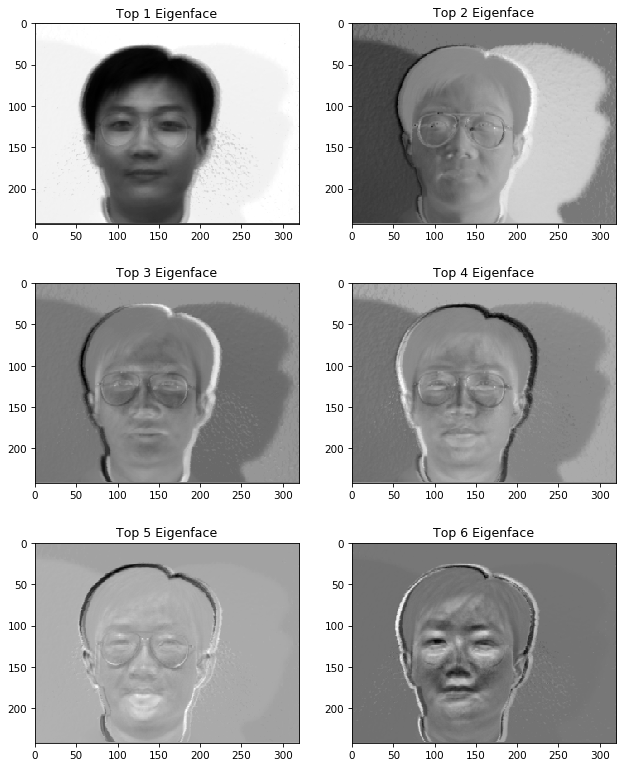
\includegraphics[scale = 0.36]{subject14.png}
\end{figure}

The top 6 eigenfaces are the most important features which characterize the global variation among face images of a subject.

Comparing the top 6 eigenfaces of subject 1 with his original images, we can see that eigenfaces clearly show his facial features: big nose, square face, deep crease on his eyes, etc.. And the top 6 eigenfaces do not show obvious emotions, such as sad or happy, which is beneficial to our recognition task. Besides, the light direction does not affect our ability to recognize his face (even though the original leftlight and rightlight pictures do make his face different). His hair is less visible in eigenfaces, which makes the recognition task easier.

Comparing the top 6 eigenfaces of subject 14 with his original images, we can see eigenfaces show his facial features very well too. We can recognize him without the glasses. And light direction does not affect our ability to recognize his face. 

\subsection{face recognition task}
The correlation between vector a and b can be calculated as $r =\frac{a^T b}{\left \| a\right \| \left \| b \right \|}$. So in this task, we compute the correlation (score) between test image and eigenfaces to see if they are close to each other. The higher the score is, the more similar they are. 

So our score is:
$$\frac{(TestImage_i)^T(FirstEigenface_i)}{\parallel TestImage_i \parallel \parallel FirstEigenface_i\parallel }$$

\medskip
Through calculation, the four scores are:

(1) projecting test image of Subject 1 using eigenface of Subject 1: \textbf{0.37}

(2) projecting test image of Subject 1 using eigenface of Subject 14: \textbf{0.12}

(3) projecting test image of Subject 14 using eigenface of Subject 1: \textbf{0.1}

(4) projecting test image of Subject 14 using eigenface of Subject 14: \textbf{0.39}

\medskip
From above scores, we can recognize the faces by scores. The test image of a subject scores higher with their respective eigenface. So test image of subject 1 is recognized as subject 1, and test image of subject 14 is recognized as subject 14.

\section{Order of faces using ISOMAP}
\subsection{Visualize the similarity graph}
Please note that the closer point i and j are, the deeper the color their edge is, e.g, darker red.

\begin{centering}
\begin{figure}[h!]
\centering
  \caption{Adjacency Matrix with weights hown using
intensity}
  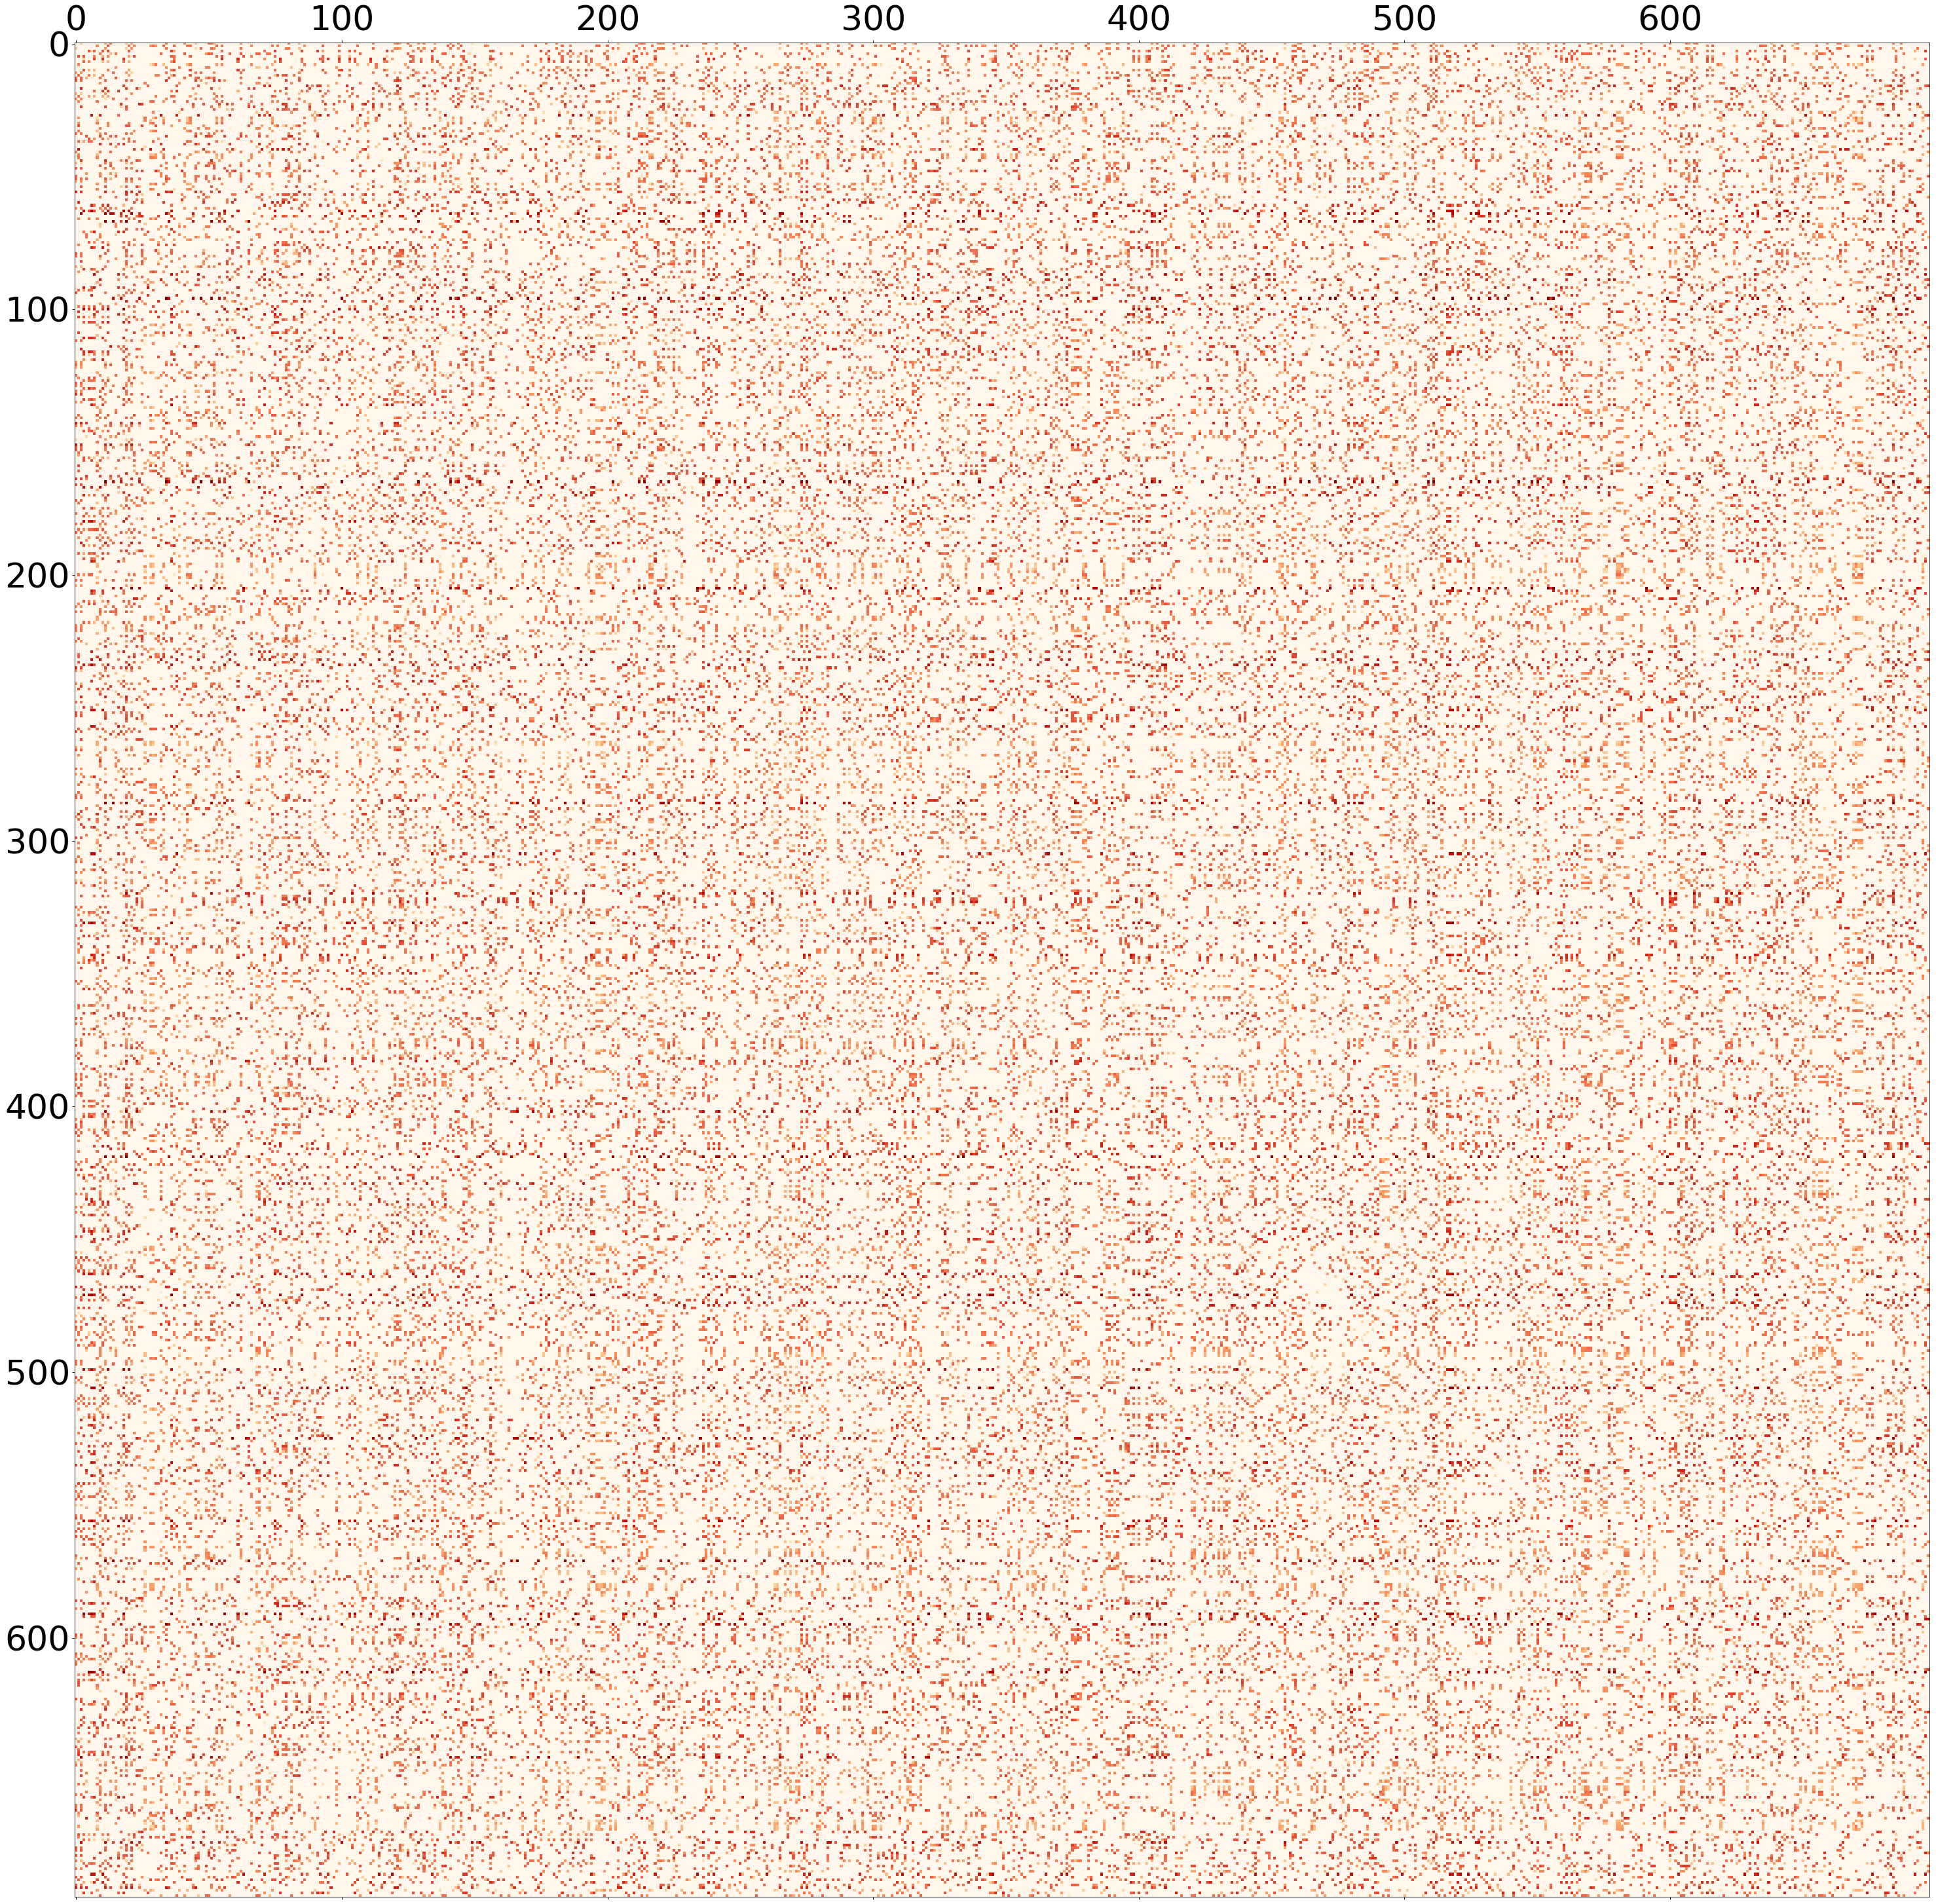
\includegraphics[scale = 0.16]{adjacency.png}
\end{figure}
\end{centering}

\subsection{2-dimensional embedding}
\begin{centering}
\begin{figure}[h!]
\centering
  \caption{2D embedding of pictures and three close faces}
  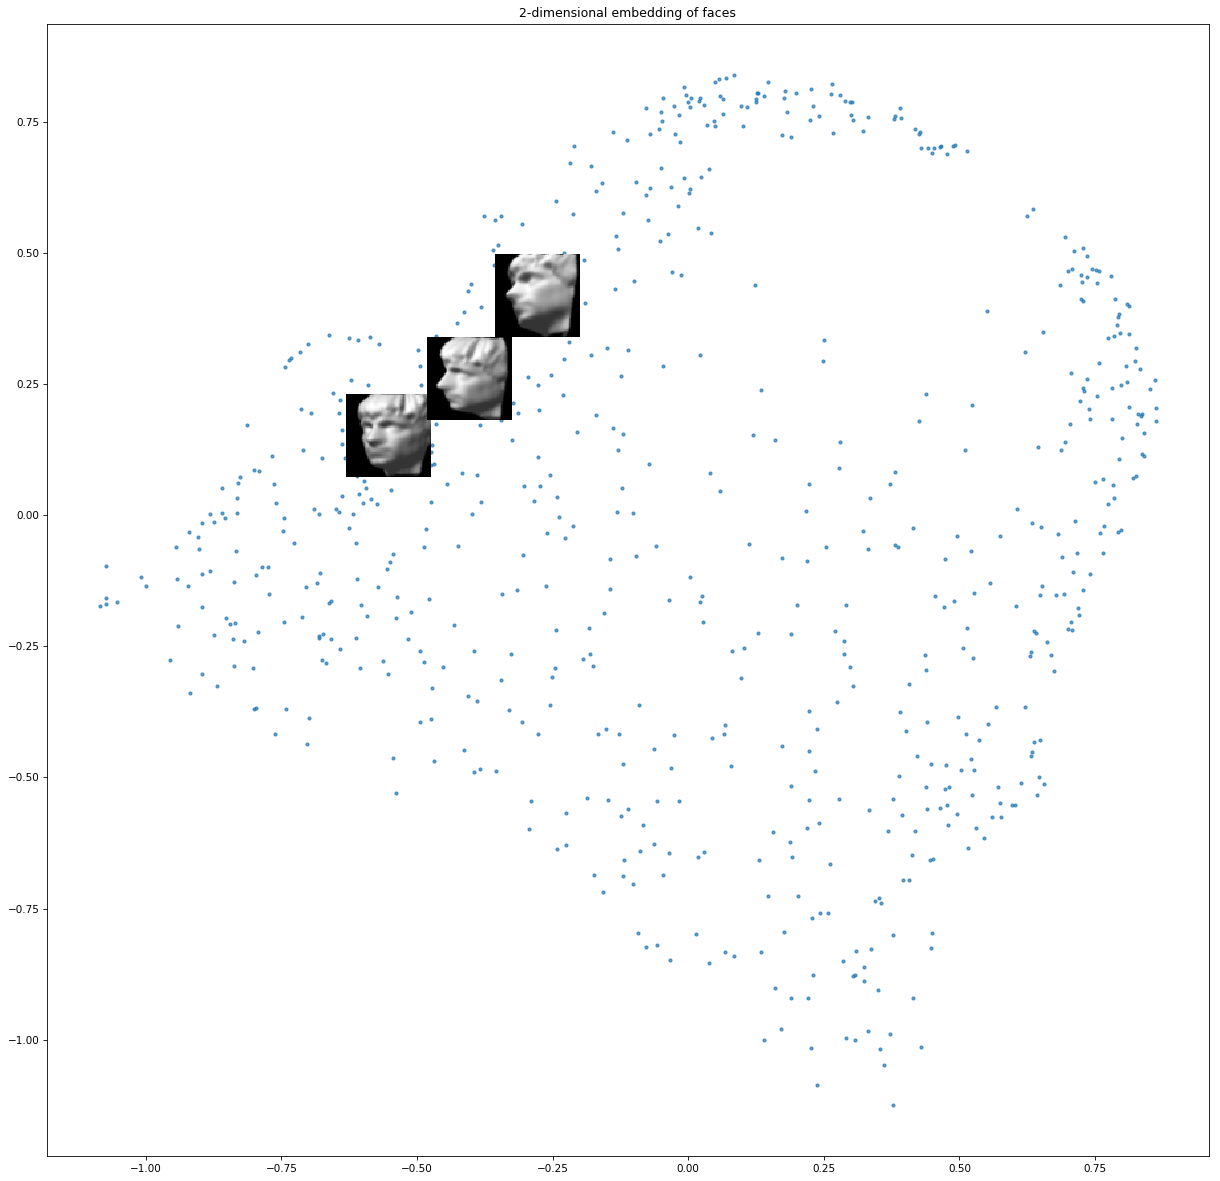
\includegraphics[scale = 0.4]{three_faces.png}
\end{figure}
\end{centering}

I choose a random image and find its two closest points in 2 dimension by minimizing their euclidean distances. We can see these three faces all facing towards left, thus they are very similar and the isomap algorithm successfully embeds these faces by their similarity.

\end{document}